\chapter{Yhteenveto}%
\label{ch:yhteenveto}

\section{Tulokset}

Koulutettu malli vaikuttaa melko käyttökelpoiselta. Tärkeimpänä tuotoksena kuitenkin ovat datasetin prosessointiin toteutetut työkalut.
Vaikka täydellistä tapaa ei löytynytkään, on lopputuloksesta silti nähtävissä, että yritetty datankäsittely on mahdollista.
Käytetyt tavat segmentoitujen alueiden poistamiseen näyttivät toimivan melko hyvin.
Erityisesti vertikaalinen pyyhkäisy arvioidun alueen ollessa kuvan keskellä tuotti hyviä tuloksia.
Koulutusdatan ominaisuuksiin perustuva "polttopisteeseen" perustuva pyyhkäisytekniikka vaikutti lupaavalta.
Ongelmia kuitenkin tuotti datan epätarkkuus.
Etenkin syvyysdata oli usein epätarkkaa segmentaatioon verrattuna.
Tämä johti tilanteisiin, joissa pyyhkäisyn alku lähti virheellisestä syvyydestä ja koko lopullinen data oli pilalla. 
Yleinen ongelma oli myös pyyhkäisyn alkaminen kuvan ulkopuolelta.
Näissäkin tilanteissa pyyhkäisyn alku saattoi alkaa väärästä syvyydestä.

Mallin tuottamat tulokset olivat melko hyviä sen oman datan kanssa.
Kuitenkin ulkopuolisen datan kanssa lopullisen mallin tuotokset ovat hyvin epätarkkoja Kuva \ref{fig:ulkoinen}.
On nähtävissä, että malli alkaa muodostua oikeaan suuntaan, mutta se tarvitsisi paljon erilaista dataa toimiakseen.

\begin{figure}[h]
\centering
\pdftooltip{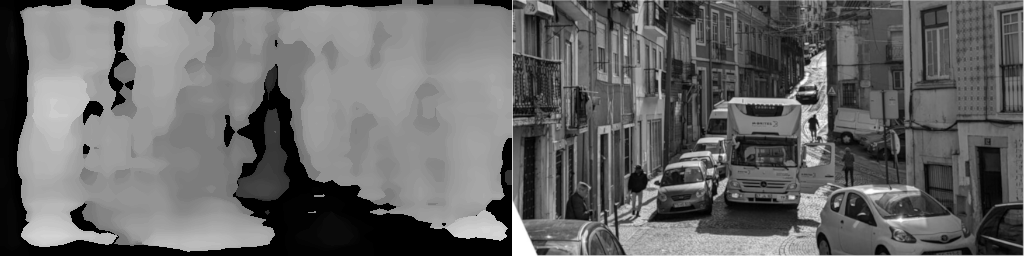
\includegraphics[width=\textwidth]{figures/outside_image.png}}{ulkoinen}
\caption{Mallin ulkopuolisista kuvista arvioitu tulos}
\label{fig:ulkoinen}
\end{figure}

Yleisesti ottaen työn tuottaman mallin tuloksiin voidaan mielestäni olla tyytyväisiä.
Jos tarve tämänkaltaiselle mallille kasvaa tarpeeksi suureksi, pystyy nyt käytetyillä tekniikoilla jalostamaan dataa melko varmasti.
Myös mallin antama "sumea" tulos on riittävän tarkka hyödyntämään esimerkiksi likimääräisten 3D-mallien sijoittamiseen kuvien päälle.

\section{Käyttökohteet}

Nykyisellään ainoa realistinen käyttökohde on itseajavien autojen ajoreittien suunnittelussa.
Mikäli olisi mahdollista saada segmentointi- ja syvyysdataa esimerkiksi ilmakuvista tai sisätiloista, voisi tätä mallia lisäkoulutuksella käyttää myös niiden skannaamiseen.

Mahdollinen ongelma tuolloin olisi sama kuin nykyiselläänkin, eli datan muokkaus.
Kuitenkin käytetyt tekniikat ja luodut skriptit pitäisi olla täysin käytettävissä minkä tahansa stereodatan kanssa.
Segmentointidatan ei tarvitse olla samasta lähteestä, jos löydetään luotettava malli tai ollaan valmiita manuaaliseen läpikäyntiin.
Kuvattavasta kohteesta riippuen nykypäivänä saatavilla olevat segmentaatiomallit voisi nähdä tarpeeksi luotettavaksi automaattiseen generointiin.

\section{Kehitysehdotukset}

Jos mallia optimoisi pienemmälle verkolle, sitä voisi ajaa suoraan esimerkiksi kuvasulaitteella.
Tämä mahdollistaisi esimerkiksi maaston skannaamisen ja datan välittömän käyttämisen laitteiden reitityksen suunnitteluun.
Mallia voisi myös parantaa, jos ajateltaisiin lähtökohtana olevan LIDAR-skannaus.
Tällöin syvyysdata voisi olla luotettavampaa, koska lähdedatalla olisi varma totuus. 

Nyt luotu malli ei ole täysin suoraan semanttista segmentaatiota.
Tästä johtuen voisi pohtia, olisiko jokin muu verkko kuin semanttiseen segmentaatioon suunniteltu parempi.
Tämä kuitenkin olisi loputon suo ja vaatisi hyvin paljon töitä,
joka kuitenkin olisi tarpeellista, jos malli halutaan ajaa edge-laitteella, kuten esimerkiksi dronella. 
Tämä voisi tehostaa toimintaa huomattavasti, koska ulostulon kokoa voitaisiin todennäköisesti pienentää melko paljon, jos jokaiselle syvyydelle ei tarvittaisi omaa segmentaatioluokkaa.

Ehkä hyödyllisin jatkokehitys olisi loppudatan lisäanalyysi.
Jos kuvien tuottamat 3D-pisteavaruudet saataisiin yhdistettyä, voitaisiin muodostaa tilojen 3D-skannauksia.
Tämä tekisi mallista oikeasti hyödyllisen ja tuotteistettavan.
Nykyisellään sen käytännön hyöty ei ole kovin suuri muuhun kuin järjestelmille, jotka erikseen tätä tarvitsevat.
Erilaisten tilojen 3D-skannaus ilman esteitä olisi hyödyllistä esimerkiksi maanmittauksessa, sisustuksessa tai kaupunkisuunnittelussa.

Suurimpia ongelmia on koulutusdatan löytäminen.
Yksi kehitysidea on rakentaa data kahden mallin avulla, 
jolloin voitaisiin käyttää mitä tahansa stereodataa, josta segmentoitaisiin objektit pois.
Tämä kuitenkin muuttuvalla taustalla hankaloittaisi suuresti datan validointia.
Jotta luotettavaa dataa saataisiin, tulisi tilasta ottaa stereokuvia ja kaikki liikkuvat kohteet poistaa,
mikä olisi kuitenkin vielä työläämpää kuin kuvien manuaalinen tekeminen tai valvonta.
Tällaisen datan rakentaminen voisi olla ehkä helpointa asettamalla staattinen stereokamera ympäristöön,
josta esimerkiksi minuutin odotuksen jälkeen voidaan automaattisesti suodattaa kaikki kuvassa liikkuneet kohteet.
Näin voitaisiin generoida melko monipuolista dataa, eikä dataa tarvitsisi edes suoranaisesti segmentöidä,
koska kuvista muihin vertaamalla olisi liikkuvien alueiden tunnistaminen helppoa.
Tämä tapa on kuitenkin melko aikaavievää, kun puhutaan tarpeesta kuvata tuhansia kuvia hyödyllisen datasetin kouluttamiseen.

Koulutusdatan muodostaminen voisi olla tehokasta videoiden perusteella.
Liikkuvasta ajoneuvosta kuvatessa pitäisi paikallaan olevien objektien tunnistamisen olla melko helppoa.
Tämän voisi yhdistää esimerkiksi 3D-mallin rakentamiseen, jolloin eri kohdista videota kerätty data voitaisiin hyödyntää kohteiden takana olevan tilan arviointiin.
Videoiden prosessointi olisi kuitenkin kuviin verrattuna hyvin erilainen prosessi,
mutta jos tällainen prosessointi saataisiin toimimaan, olisi sille datan hankkiminen hyvin helppoa.
Teoriassa staattisten kohteiden tunnistaminen olisi helppoa, koska ne jäisivät kuvassa koko ajan taustalle,
ja syvyyden arviointi voitaisiin suorittaa likimääräisesti ilman stereokameraa, koska samoista kohteista olisi useita kuvia.
Näiden kohteiden sijoitus kuvissa sekä auton nopeusdatan analysointi mahdollistaisi dispariteettianalyysin.
Tai mikäli jos ajoneuvo olisi varustettu LIDAR:illa, voitaisiin suurin osa työstä tehdä suoraan pisteavaruuksia käsittelemällä.

Vaihtoehto olisi myös generoida data tietokoneella graafisesti,
mutta se toisi omat tekniset ongelmansa ja sen hyödyntäminen oikeassa maailmassa voisi olla melko rajallista.
Tämä vaihtoehto vaatisi paljon testaamista.
Datan tuottaminen itsessään olisi melko helppoa
ja esikäsitelty kuva voisi olla tarpeeksi samankaltainen generoitujen kuvien kanssa.
